% -*- mode : latex; coding: utf-8 -*-
\chapter{Evaluation} \label{sec:Evaluation}

This chapter deals with workloads and configuration I used for simulation, and compares storage overhead and performance result
between the normal and optimized version of Graphene and Hydra. 
\section{Experimental Setup} \label{sec:exp-setup}
\subsection{Simulator Setup}
\label{sec:simulator-setup}

I implemented Graphene, Hydra, and optimized versions in Macsim \cite{MACSIM} with Ramulator \cite{RAMULATOR}, 
a cycle-accurate trace-driven simulator. I consider NRR as successive activation of two rows and modified Ramulator 
to support NRR command with timing parameters set accordingly. 
I configured Ramulator to follow the organization of the Micron DDR4 8Gb x8 chip and set ACT, PRE, RD, and WR timing accurately. 
Table \ref{tab:Sim_setting} shows the detailed experimental configuration for Ramulator and Macsim. 

\subsection{Workload Setup}
\label{sec:workload-setup}
I evaluate baseline Graphene, Hydra, and each optimized version using 2 synthetic attack patterns and 3 normal workloads from
SPEC2017 rate benchmark\cite{SPEC2017}. The three most memory-intensive benchmarks were chosen according to workload 
characterization in Hydra: parest, blender, and cactuBSSN. These benchmarks showed the highest number of 
unique rows which received more than 250 ACTs during tREFW. To compare the performance of different designs under RH attack, 
two synthetic attack patterns were used: Repetitively accessing two rows apart far from each other and double-hammering attack. 

\begin{table}[t]
\centering
  \caption{Simulation setting of Macsim and Ramulator}
  \label{tab:Sim_setting}
  \begin{tabular}[width=\textwidth]{|c|c|c|}
  \toprule
    \multicolumn{2}{|c|}{MACSIM CPU Configuration} \\
  \midrule 
    Core &  4-core \@ 3.2GHz \\ 
    Private L1 Cache (set-way) &  Icache 4KB (8-8), Dcache 16KB (32-8) \\
    Private L2 Cache (set-way) & 128KB (128-16) \\
    Shared LLC (set-way) & 1MB (1024-16) \\
    Trace maximum & 80M \\
  \toprule
    \multicolumn{2}{|c|}{Ramulator Memory Configuration} \\
  \midrule 
    Speed & DDR4-2400R \\ 
    Memory bus speed & 12GHz (2.4GHz DDR) \\
    Organization & DDR4 8Gb x8 \\ 
    Configuration & 2ch-1ra-4bg-4ba \\
    Capacity & 16Gb \\
    Scheduling &  FCFS \\
    Row Policy & Opened row \\
    $Flip_{th}$ & 1K \\
    Hydra-op $Flip_{th}$ distribution & Uniform [1K, 21K] \\
  \bottomrule
  \end{tabular}
\end{table}

\section{Evaluation Result}
\label{sec:evaluation-result}

\subsection{Storage Overhead}
\label{sec:storage-overhead}

\begin{wraptable}{R}{8cm}
  \caption{Storage Overhead}
  \label{wrap-tab:Storage}
  \begin{tabular}{|c|c|c|}
  \toprule
    Design & Storage size (Byte) & Type \\
  \midrule 
    Graphene & 533,400 & CAM \\ \hline
    Graphene-op & 554,736 & CAM \\ \hline
    \multirow{2}{*}{Hydra} & 56,576 & SRAM \\ 
       & 2,097,152 (0.1\%) & DRAM \\ \hline
    \multirow{2}{*}{Hydra-op} & 66,560 & SRAM \\ 
       & 4,194,304 (0.2\%) & DRAM \\ 
  \bottomrule
  \end{tabular}
\end{wraptable}

Table \ref{wrap-tab:Storage} shows the storage overhead of 4 designs. Increased CAM size in Graphene-op is because
it uses doubled threshold compared to Graphene and thus bit-width of the counter is increased accordingly. For Hydra-op, I assumed
each row's $Flip_{th}$ is a random variable with a distribution of uniform [1K, 21K] and saved each value alongside the counter in RCT using
the same bit-width. Thus, DRAM storage is doubled but still negligible (0.2\%) compared to the total size of DRAM used in the simulation.
In addition, each RCC entry is extended to save each row's threshold metadata, leading to a 17\% increase in total size. 

\subsection{Overall Performance}
\label{sec:overall-performance}
To comprehensively evaluate the performance of optimized versus non-optimized versions, 
I first evaluate the number of refresh actions triggered by RH mitigation schemes in malicious workloads. 
Figure \ref{fig:NRR num} shows the number of RH refreshes in each of four designs for 2 independent row hammering (\ref{fig:Single-side}) 
and double-hammering (\ref{fig:Double-side}) \footnote{Due to random distribution of each row's $Flip_{th}$, 
simulation of Hydra-op is repeated 100 times and used average}. Regardless of the attack pattern, the number of refreshes in 
Graphene-op is reduced by 50\%. This is because Graphene-op uses twice the larger threshold than Graphene.
 In the case of Hydra-op, the number of refreshes is reduced by 91.4\%. This is because the number of refreshes is inversely 
 proportional to the predefined threshold and the average threshold of Hydra-op is 11$\times$ of non-optimized Hydra. 

\begin{figure}
\centering
\begin{subfigure}[t]{.5\textwidth}
  \centering
  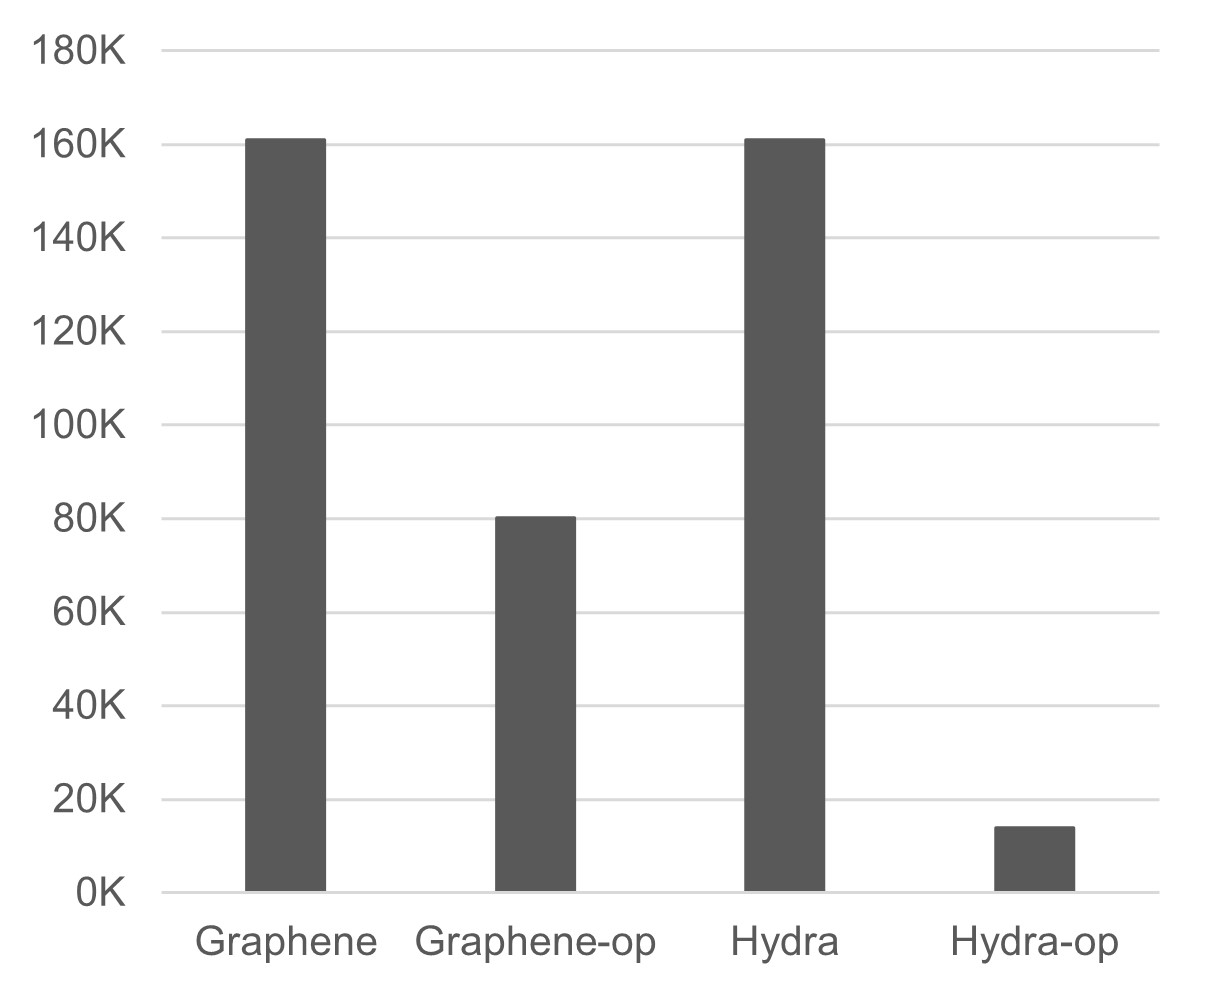
\includegraphics[width=.9\linewidth]{figures/Single sided.jpg}
  \caption{2 independent access}
  \label{fig:Single-side}
\end{subfigure}%
\begin{subfigure}[t]{.5\textwidth}
  \centering
  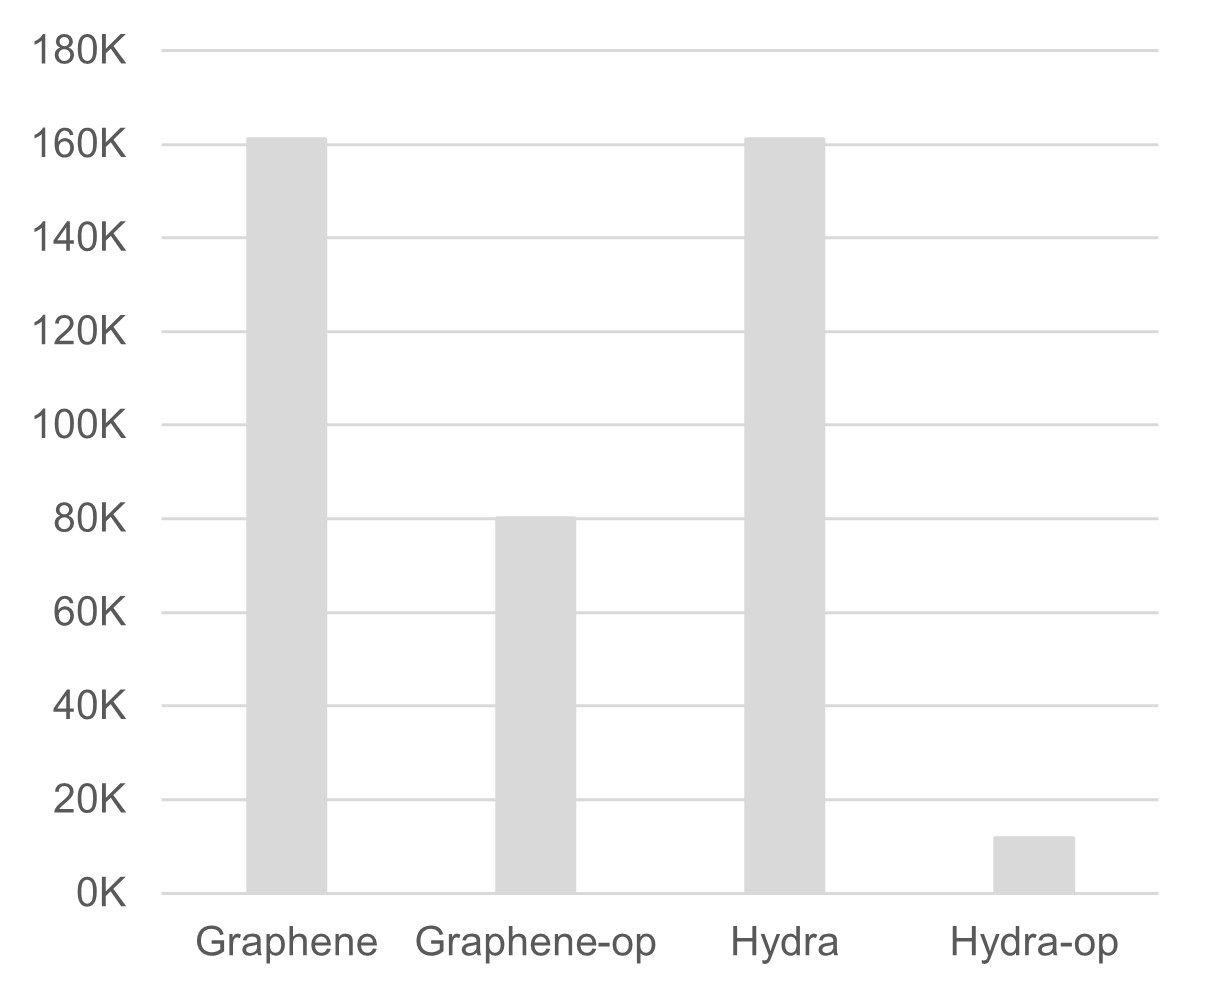
\includegraphics[width=.9\linewidth]{figures/Double sided.jpg}
  \caption{Double-hammer attack}
  \label{fig:Double-side}
\end{subfigure}
\caption{The number of refreshes as mitigation in two synthetic workloads}
\label{fig:NRR num}
\end{figure}

\begin{figure}[ht]
  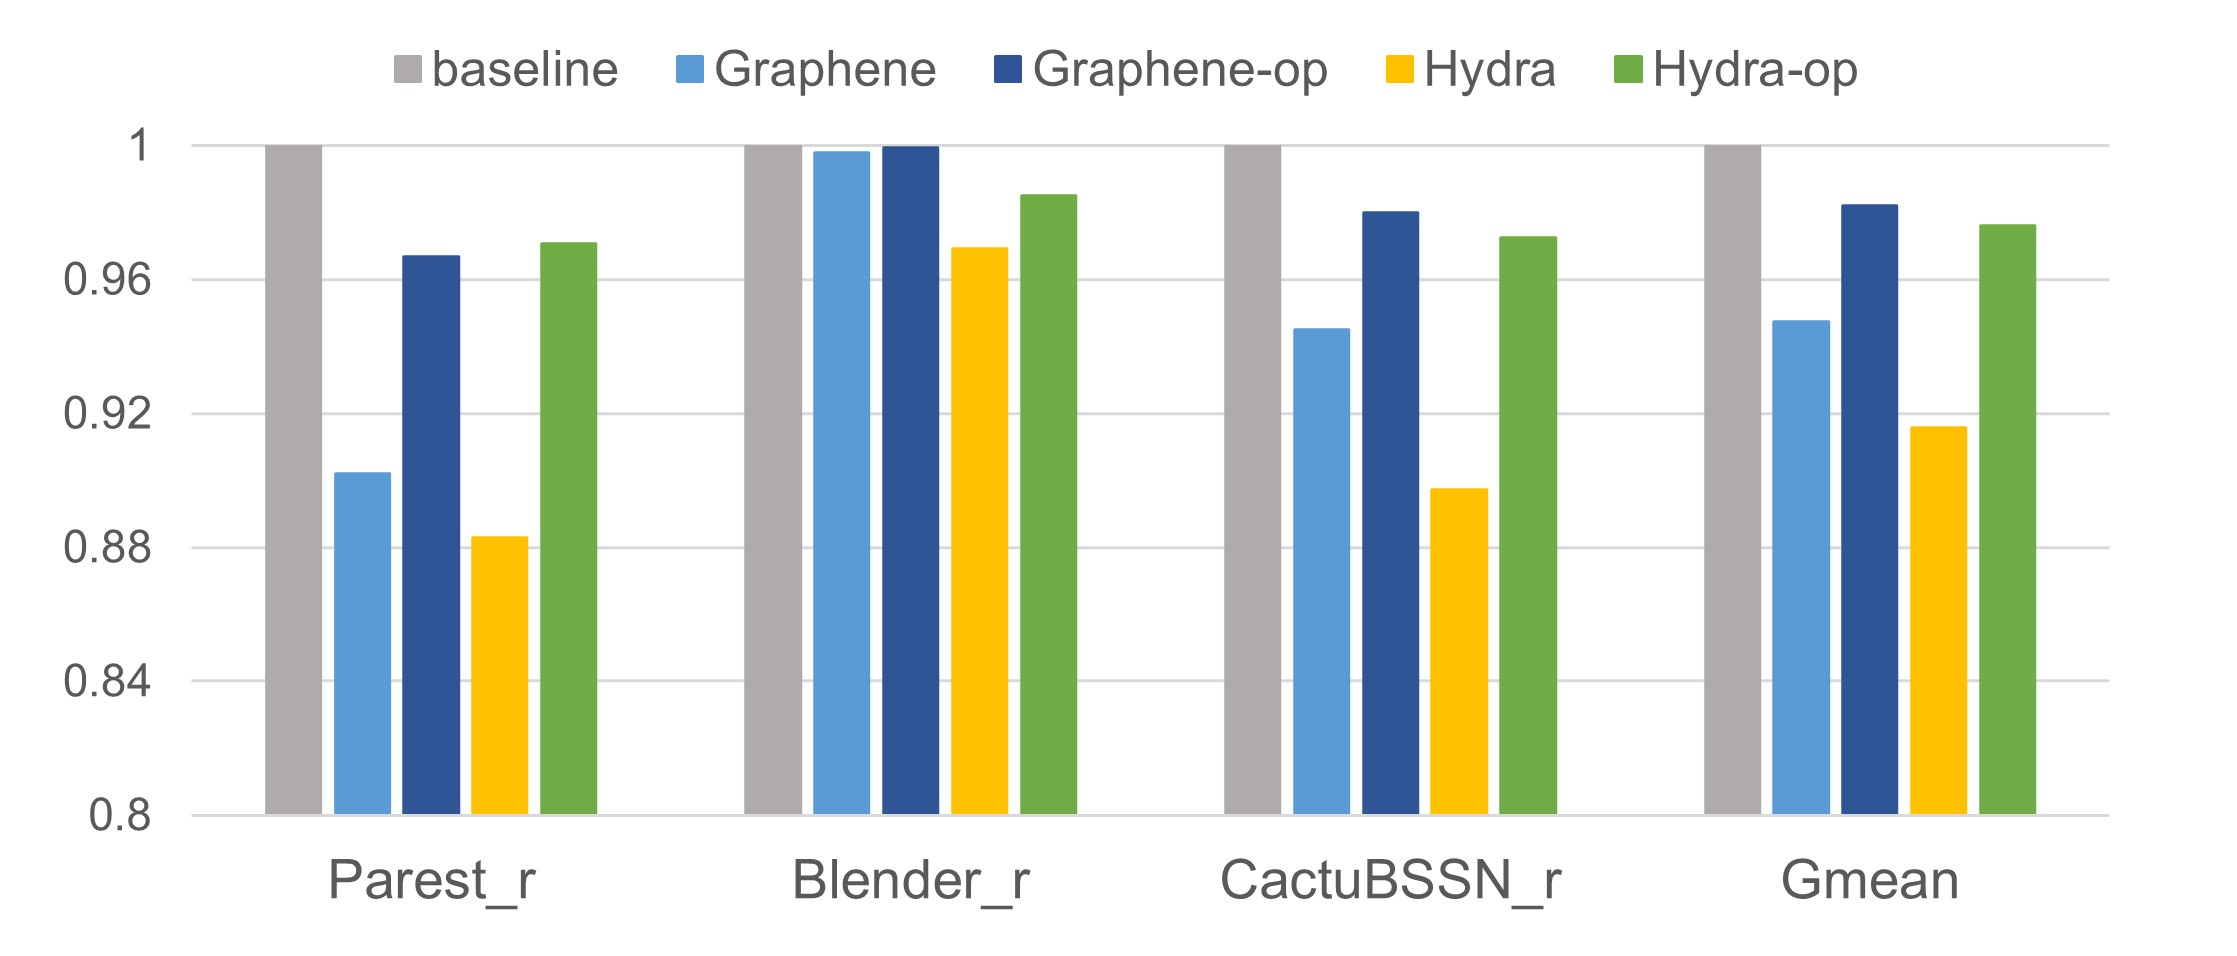
\includegraphics[width=\textwidth]{figures/Norm IPC.jpg}
  \caption{IPC normalized to baseline (no mitigation) in SPEC2017 memory-intensive workloads}
\label{fig:IPC}
\end{figure}

In the case of benign accesses, I evaluate the IPC of memory-intensive workloads explained in \ref{sec:workload-setup} for 4 designs.
Figure \ref{fig:IPC} shows IPC normalized to baseline (no RH mitigation scheme implemented). Both optimized versions of Graphene and Hydra
showed reduced performance overhead. In Graphene-op, average performance overhead is reduced by 65.7\%. This implies that tracking victims
effectively filters unnecessary refresh actions in Graphene. In the case of Hydra-op, the average performance overhead is reduced by 71.7\%. 
This shows that using per-row threshold increases effective $Flip_{th}$, leading to a smaller number of refresh actions. 

To understand the source of performance gain, further analyses are done for overhead in designs. Figure \ref{fig:Overhead}
shows additional refresh done to restore charge in victims (\ref{fig:Row Refreshes}), and extra DRAM accesses for the RCT counter in 
Hydra (\ref{fig:Extra accesses}). For Graphene, the average number of extra refreshes is reduced by 64.7\%, which matches the percentage
of reduced performance overhead. The average number of extra refreshes in Hydra is reduced by 98.1\%. However, even though extra refreshes
 were reduced by a significant amount, there were little or no performance benefits in the case of the tracker (\ref{fig:Extra accesses}) and
 showed a larger number of extra DRAM read/write. The main reason for such performance overhead is that the sum of the RCT entry size is
 doubled due to the row's $Flip_{th}$ metadata using the same bit width as the RCT counter. Extra DRAM read/write occurs when a GCT counter
 becomes $T_{G}$, and all RCT counters are initialized to $T_{G}$. Nevertheless, Hydra-op still achieves higher performance because it does 
 very few refreshes.
 
\begin{figure}
\centering
\begin{subfigure}[t]{.5\textwidth}
  \centering
  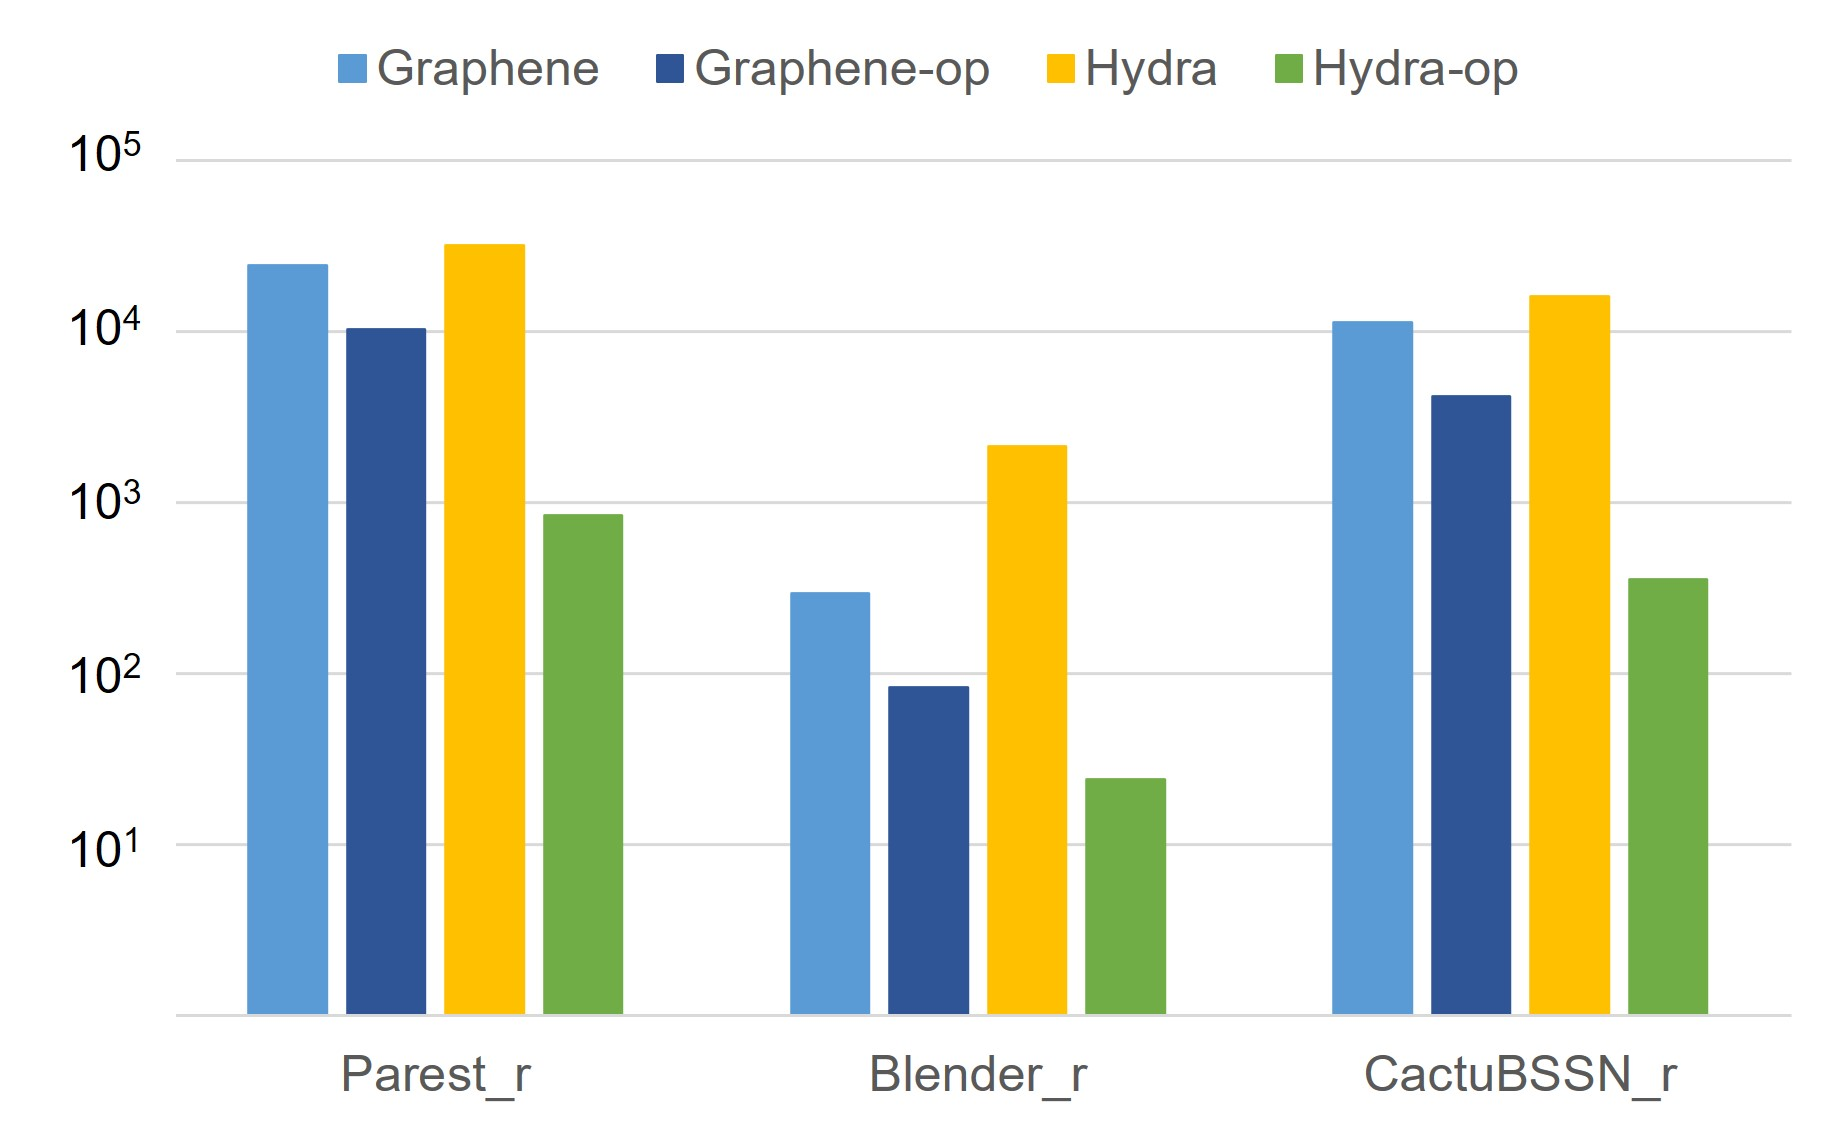
\includegraphics[width=\linewidth]{figures/Row Refreshes.jpg}
  \caption{Additional row refreshes by mitigation}
  \label{fig:Row Refreshes}
\end{subfigure}%
\begin{subfigure}[t]{.5\textwidth}
  \centering
  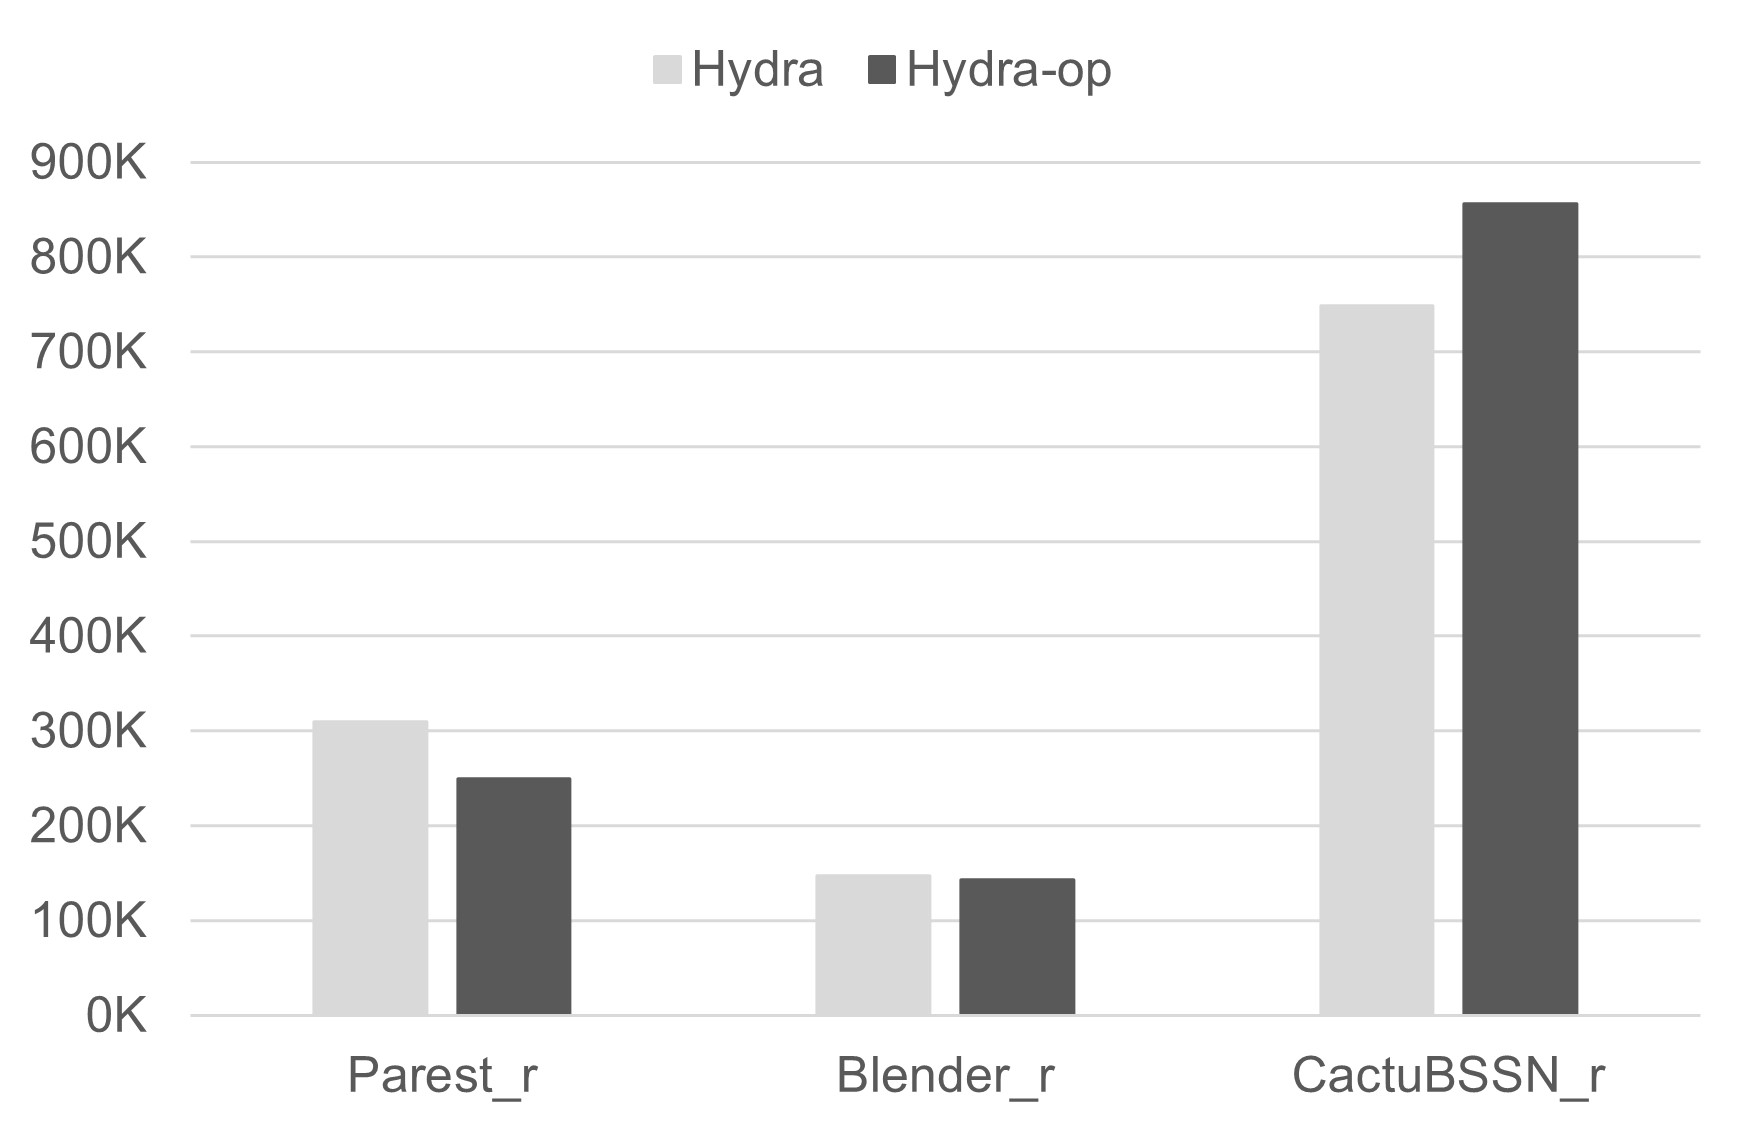
\includegraphics[width=\linewidth]{figures/Extra DRAM Acess.jpg}
  \caption{Extra DRAM accesses in Hydra, Hydra-op}
  \label{fig:Extra accesses}
\end{subfigure}
\caption{Overhead analysis in SPEC2017 workloads}
\label{fig:Overhead}
\end{figure}
